\subsection{Sortowanie przez scalanie}
Jest to rekurencyjny algorytm sortowania danych, stosujący metodę ,,dziel i zwyciężaj''. W algorytmie wyróżnia się trzy podstawowe kroki: podział danych wejściowych na 2 rozłączne podzbiory; rekurencyjnie zastosowanie sortowania dla każdego podzbioru, aż do uzyskania struktur jednoelementowych; scalenie posortowanych podzbiorów w jeden zbiór. Całkowita złożoność obliczeniowa dla sortowania przez scalanie wynosi $O(n \cdot log n)$, w związku z czym zastosowanie tego sortowania okaże się wydajniejsze dla bardzo dużych tablic.


\subsection{Sortowanie szybkie}
Również jest to algorytm sortowania danych stosujący metodę ,,dziel i zwyciężaj'', nie wykorzystuje on jednak dodatkowych podtablic. Istnieje wiele implementacji sortowania szybkiego, jednak generalna idea jest taka, że wybierany jest jeden element w sortowanej strukturze, który nazywany jest piwotem. Może być to element środkowy, pierwszy, ostatni bądź losowy, przy czym należy pamiętać, że w przypadkach, kiedy piwot jest ciągle maksymalny lub minimalny, występuje najgorsza złożoność obliczeniowa $O(n^2)$. Przy optymalnych wyborach piwotu, złożoność wynosi $O(n \cdot log n)$. 


\subsection{Sortowanie introspektywne}
Jest to odmiana sortowania hybrydowego, które opiera się na spostrzeżeniu, że niewydajne jest wywoływanie ogromnej liczby rekurencji dla małych tablic w algorytmie sortowania szybkiego. Głównym założeniem algorytmu sortowania introspektywnego jest zatem wyeliminowanie problemu złożoności $O(n^2)$ występującej w najgorszym przypadku sortowania szybkiego. Sortowanie introspektywne jest połączeniem sortowania szybkiego i sortowania przez kopcowanie, które jest traktowane jako pomocnicze. Tym samym złożoność obliczeniowa wynosi $O(n \cdot log n)$.


\subsection{Porównanie złożoności obliczeniowych wybranych algorytmów}

Poniższa tabela zestawia oczekiwane i najgorsze przypadki złożoności wybranych algorytmów sortowania. Poniżej dodano także poglądowy wykres funkcji, na którym widać, że dla małej liczby danych sortowanie o złożoności kwadratowej będzie wydajniejsze niż dla logarytmicznej i przeciwnie dla dużej liczby elementów do posortowania.

\begin{table}[H]
    \centering
    \renewcommand{\tablename}{Tab.}
    \caption{Porównanie oczekiwanych i najgorszych przypadków złożoności obliczeniowej dla wybranych algorytmów sortowania}
    \label{tab: opis_zlozonosc}
    \begin{tabular}{c|ccc|}
        \cline{2-4}
        & \multicolumn{3}{c|}{sortowanie}   \\ \cline{2-4} & \multicolumn{1}{c|}{przez scalanie} & \multicolumn{1}{c|}{szybkie} & introspektywne \\ \hline
        \multicolumn{1}{|c|}{typowa złożoność} & \multicolumn{1}{c|}{$O(nlong)$} & \multicolumn{1}{c|}{$O(nlogn)$} & $O(nlogn)$       \\ \hline
        \multicolumn{1}{|c|}{najgorszy przypadek złożoności} & \multicolumn{1}{c|}{$O(nlogn)$} & \multicolumn{1}{c|}{$O(n^2)$} & $O(nlogn)$       \\ \hline
    \end{tabular}
\end{table}

\begin{figure}[H]
    \centering
    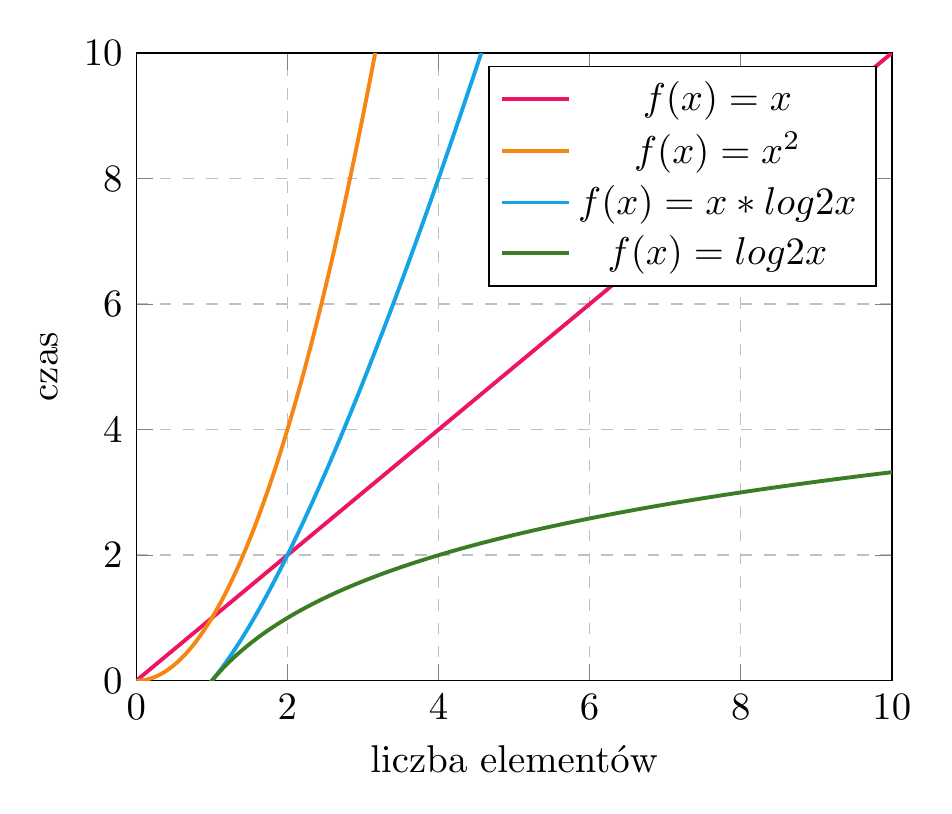
\begin{tikzpicture}[scale=1.4]
        \begin{axis}
            [
                /pgf/number format/.cd,use comma,1000 sep={},   %europejski format
                % width={\textwidth},
                % height={\textheight},
                % scale only axis=true,
                ylabel={czas},
                xlabel={liczba elementów},
                xmin=0, xmax=10,
                ymin=0, ymax=10,
                ymajorgrids=true, xmajorgrids=true, grid style=dashed
            ]
        \addplot[color=WildStrawberry, samples=1000, line width=1pt, domain=0:30] {x};
        \addplot[color=BurntOrange, samples=1000, line width=1pt, domain=0:30] {x^2};
        \addplot[color=Cerulean, samples=1000, line width=1pt, domain=0:30] {x*log2 x};
        \addplot[color=OliveGreen, samples=1000, line width=1pt, domain=0:30] {log2 x};
        \legend {$f(x)=x$ \\ $f(x) = x^2 $ \\ $f(x)=x*log2 x$ \\ $f(x)=log2 x$ \\};
        \end{axis}
    \end{tikzpicture}
    \renewcommand{\figurename}{Rys.}
    \caption{}
    \label{fig: }
\end{figure}


